% RA-L / ICRA 2027 submission
% Compiled with: pdflatex rover_nav_paper.tex (twice for refs)
\documentclass[letterpaper, 10pt, journal]{IEEEtran}

\usepackage[T1]{fontenc}
\usepackage[utf8]{inputenc}
\usepackage{amsmath,amssymb}
\usepackage{graphicx}
\usepackage{booktabs}
\usepackage{url}
\usepackage{hyperref}
\usepackage{xcolor}
\usepackage{algorithm}
\usepackage{algorithmic}
\usepackage{microtype}

\hypersetup{colorlinks=true, linkcolor=blue, citecolor=blue, urlcolor=blue}

% --------------------------------------------------------------------------- title
\title{Reactive Ground Rover Navigation via Recurrent Reinforcement Learning
       with 360\textdegree{} Lidar}

\author{Yusuf~Saib%
  \thanks{Y.~Saib is with Coybot (\texttt{yusuf@coybot.ai}).
  This work was conducted on privately owned hardware.
  Code is available at \url{https://github.com/coybot-ai/rover-nav-rl}.}}

\markboth{IEEE Robotics and Automation Letters,~Vol.~XX, No.~XX, 2027}%
{Saib: Reactive Ground Rover Navigation via Recurrent RL with 360\textdegree{} Lidar}

\begin{document}
\maketitle

% --------------------------------------------------------------------------- abstract
\begin{abstract}
We present a learned reactive navigation policy for differential-drive ground robots
that achieves zero-collision traversal of cluttered environments and multi-wall mazes
using only 360\textdegree{} lidar and odometry---no map, no global planner, no
demonstrations.
The policy is a recurrent actor-critic (GRU, hidden size 256) trained with Proximal
Policy Optimisation (PPO) across 512 parallel GPU-vectorised environments.
A four-stage curriculum advances from open-field goal-seeking to dense obstacle fields
and tight slalom gauntlets, with domain randomisation covering wheel lag, control
latency, sensor noise, and heading drift throughout.
Training from scratch requires approximately 30 minutes on a dual-RTX-5090 workstation.
The exported ONNX policy weighs 4.6~KB and runs in carry-state step-mode---a single
83-dimensional observation plus a 256-float GRU hidden state per call---enabling
10~Hz deployment on a Jetson Orin Nano with negligible compute overhead.
Evaluated on six named courses across 20 noisy trials each
(RPLidar noise $\sigma{=}0.05$~m, odometry $\sigma{=}0.10$~m),
the policy achieves 100\% goal-reach with zero collisions across 120 trials.
A Vector Field Histogram (VFH) baseline run on identical conditions
achieves 83\% reach (100/120) and fails entirely on cluttered fields (0/20 reach,
20/20 collisions), demonstrating a qualitative capability gap in dense, unstructured
environments.
We report the full reward formulation, curriculum schedule, architecture, and training
dynamics, and release all code for reproducibility.
\end{abstract}

\begin{IEEEkeywords}
mobile robot navigation, reinforcement learning, recurrent policy, lidar,
obstacle avoidance, sim-to-real, curriculum learning
\end{IEEEkeywords}

% --------------------------------------------------------------------------- I. intro
\section{Introduction}

Reactive obstacle avoidance for ground robots is a fundamental problem in mobile
robotics: given only onboard sensors, navigate from a start pose to a goal without
hitting anything. Classical approaches---Vector Field Histogram~\cite{vfh},
Dynamic Window Approach~\cite{dwa}, and their descendants---build explicit local
representations of free space and select actions by optimising hand-crafted cost
functions. They are interpretable and fast, but their performance degrades in dense,
cluttered environments where the histogram is ambiguous and local minima are common.

Learning-based methods offer an alternative: replace the hand-crafted planner with a
policy trained to maximise cumulative reward, letting the agent discover avoidance
strategies without requiring a closed-form model of the environment. Recent work has
demonstrated effective learned navigation from cameras~\cite{shah2023gnm},
lidar~\cite{tai2017virtual, zhelo2018curiosity}, and fused
representations~\cite{fang2019scene}, but often requires large offline datasets,
human demonstrations, or map-based auxiliary objectives.

This paper asks: how far can a \emph{purely reactive} policy go---one that sees only
lidar ranges and a body-frame goal vector, carries no map, and was trained with no
demonstrations? Our answer is: surprisingly far. We present a lightweight recurrent
PPO agent that trains end-to-end in 30 minutes and navigates six qualitatively
distinct 2D obstacle courses, including tight-gap traversal and four-room maze
exploration, with 100\% success and zero collisions under realistic sensor noise.

\textbf{Contributions:}
\begin{enumerate}
  \item A complete, reproducible training recipe for reactive ground rover navigation:
    reward formulation, four-stage curriculum, domain randomisation schedule,
    architecture, and ONNX deployment format.
  \item Empirical demonstration that a recurrent policy (GRU) substantially
    outperforms a reactive analytic baseline (VFH) on dense obstacle fields, while
    matching it on structured courses---with a 4.6~KB policy that runs at 10~Hz on
    edge hardware.
  \item Analysis of the training dynamics: the policy reaches 100\% success at
    deployment despite training-time reach of only 45--56\% on the hardest curriculum
    stage, suggesting that hard-stage curriculum training builds robustness beyond
    what in-training metrics reveal.
  \item A characterisation of key design decisions---360\textdegree{} vs.\ forward
    lidar, GRU vs.\ MLP, separate actor/critic recurrent states---with qualitative
    evidence for each.
\end{enumerate}

% --------------------------------------------------------------------------- II. related
\section{Related Work}

\subsection{Classical Reactive Navigation}

The Vector Field Histogram~\cite{vfh} and its successor VFH+~\cite{vfhplus}
represent the dominant analytic reactive planning family: a polar obstacle-density
histogram is built from sonar or lidar data, free sectors are identified by
thresholding, and the planner steers toward the sector nearest the goal direction.
The Dynamic Window Approach~\cite{dwa} instead samples feasible velocity commands
and selects those maximising a composite score of goal alignment, clearance, and
speed. Both methods are memoryless---they act on the current sensor snapshot---and
are susceptible to local minima in dense or symmetric environments.

\subsection{Learned Navigation with Lidar}

Tai et al.~\cite{tai2017virtual} demonstrated sim-to-real transfer of a
lidar-conditioned policy for hallway navigation using an asynchronous deep RL
framework. Zhelo et al.~\cite{zhelo2018curiosity} combined intrinsic curiosity with
a lidar-based policy for exploration. Neither work evaluates against analytic baselines
on identical courses, nor reports systematic noise stress-tests. Our work contributes
a direct comparison with VFH on shared, reproducible courses under matched noise.

\subsection{Recurrent Policies for Partial Observability}

The benefits of recurrent policies for partially observable navigation have been
established in simulation~\cite{mirowski2016learning, zhu2017target} and increasingly
on physical hardware~\cite{kahn2021badgr}. Our work confirms that GRU memory is
beneficial even for a \emph{ground} rover with 360\textdegree{} sensing: the history
encodes velocity integration and past heading choices, enabling the policy to break
symmetry in locally ambiguous scenes and recover from near-miss states.

\subsection{Curriculum and Domain Randomisation for Sim-to-Real}

Curriculum learning~\cite{bengio2009curriculum} and domain
randomisation~\cite{tobin2017domain} are now standard ingredients in robot learning.
OpenAI's dexterous manipulation work~\cite{openai2019dexterous} demonstrated that
progressive difficulty and aggressive randomisation can bridge the sim-to-real gap for
complex contact-rich tasks. We apply both principles to reactive navigation, scheduling
domain randomisation to activate only after the base policy is stable, and advancing
curriculum stages at fixed fractional milestones rather than adaptive thresholds.

% --------------------------------------------------------------------------- III. problem
\section{Problem Formulation}

We consider a differential-drive ground robot (the ``rover'') operating in a 2D
planar environment cluttered with axis-aligned box obstacles. At each timestep $t$,
the rover receives a 360\textdegree{} lidar scan $\mathbf{l}_t \in \mathbb{R}^{72}$,
body-frame odometry $(v_t, \omega_t)$, and a body-frame vector to a fixed goal
$\mathbf{g}_t \in \mathbb{R}^2$. It outputs a velocity command
$\mathbf{a}_t = [v^{\mathrm{cmd}}_t, \omega^{\mathrm{cmd}}_t]$ that is applied via
unicycle integration.

The goal is to find a policy $\pi$ that navigates from any start pose within a
training distribution to the goal within a time budget, while maintaining a minimum
clearance $d_{\min} > r_{\mathrm{body}}$ from all obstacles. The policy must be
purely reactive: it has no access to a map, no prior knowledge of obstacle geometry,
and no global planner. At deployment, the full observation history is summarised in
the GRU hidden state $\mathbf{h}_t$ carried across calls.

% --------------------------------------------------------------------------- IV. method
\section{Method}

\subsection{Observation Space}

The 83-dimensional observation vector is defined as follows (body frame throughout):

\begin{equation}
\mathbf{s}_t = \bigl[
  g^{\mathrm{fwd}},\; g^{\mathrm{left}},\; 0,\; \|\mathbf{g}_t\|,\;
  v_t,\; 0,\; 0,\; \psi_{\mathrm{err}},\; \omega_t,\; 0,\; 1.0,\;
  l_t^{(0)},\ldots,l_t^{(71)}
\bigr]
\end{equation}

\noindent where $g^{\mathrm{fwd}}, g^{\mathrm{left}}$ are the body-frame goal
components, $\psi_{\mathrm{err}} \in (-\pi, \pi]$ is the heading error to the goal,
and $l_t^{(i)}$ is the range of the $i$-th lidar ray (72 rays at $5^\circ$ spacing,
capped at 10~m). Constant-zero slots maintain a fixed-width interface shared with the
aerial policy architecture from which this design was adapted. A vehicle-type flag
(1.0 for rover) occupies slot~10. Mean/std normalisation constants are baked into the
ONNX graph at export so callers pass raw unnormalised observations.

\subsection{Action Space}

The two-dimensional continuous action $\mathbf{a}_t = [v^{\mathrm{cmd}}, \omega^{\mathrm{cmd}}]$
maps directly to a ROS2 \texttt{/cmd\_vel} Twist message
(linear.x~$= v^{\mathrm{cmd}}$, angular.z~$= \omega^{\mathrm{cmd}}$), clipped to
$v \in [-2.0, 2.0]$~m/s and $\omega \in [-2.0, 2.0]$~rad/s.
This matches unicycle kinematics exactly: no lateral velocity, no altitude.
Matching the action space to hardware kinematics reduces exploration dimensionality
and eliminates the need for a post-hoc kinematic projection layer.

\subsection{Reward Function}

The reward at each timestep is a sum of dense shaping and sparse terminal terms:

\begin{equation}
r_t = \underbrace{k_{\mathrm{prog}} \cdot \Delta d}_{\text{progress}}
    - \underbrace{k_{\mathrm{time}}}_{\text{time}}
    - \underbrace{k_{\mathrm{jerk}} \|\Delta\mathbf{a}\|}_{\text{smoothness}}
    - \underbrace{k_{\mathrm{stall}} \cdot \mathbf{1}[v < 0.2]}_{\text{stall}}
    - \underbrace{k_{\mathrm{clear}} \cdot \max(0,\, m - d_{\min})}_{\text{proximity}}
    + \underbrace{k_{\mathrm{goal}} \cdot \mathbf{1}[\text{reached}]}_{\text{goal}}
    - \underbrace{k_{\mathrm{coll}} \cdot \mathbf{1}[\text{collision}]}_{\text{collision}}
    - \underbrace{k_{\mathrm{to}} \cdot \mathbf{1}[\text{timeout}]}_{\text{timeout}}
\end{equation}

\noindent with weights $k_{\mathrm{prog}}{=}1.5$, $k_{\mathrm{time}}{=}0.03$,
$k_{\mathrm{jerk}}{=}0.003$, $k_{\mathrm{stall}}{=}0.3$,
$k_{\mathrm{clear}}{=}0.6$, margin $m{=}0.5$~m,
$k_{\mathrm{goal}}{=}40$, $k_{\mathrm{coll}}{=}25$, $k_{\mathrm{to}}{=}10$.

The \emph{proximity penalty} is the critical term for clearance behaviour: it fires a
running per-tick cost whenever the rover's minimum obstacle clearance $d_{\min}$ drops
below $m = 0.5$~m, well before the collision threshold of 0.3~m. Without this term,
the policy learns to graze obstacles (collision fires only at contact; incidental
proximity is free). With it, the policy maintains buffer distances as a systematic
strategy, visible in the mean clearances of Table~\ref{tab:results}.

\subsection{Architecture}

The policy is a \emph{separate} actor-critic recurrent network:

\begin{equation}
\begin{aligned}
\mathbf{h}^{\pi}_{t} &= \mathrm{GRU}_{256}^{\pi}\!\left(\mathrm{Norm}(\mathbf{s}_t),\,\mathbf{h}^{\pi}_{t-1}\right),\quad
\mathbf{a}_t \sim \pi_\theta\!\left(\cdot \mid \mathbf{h}^{\pi}_{t}\right) \\
\mathbf{h}^{V}_{t} &= \mathrm{GRU}_{256}^{V}\!\left(\mathrm{Norm}(\mathbf{s}_t),\,\mathbf{h}^{V}_{t-1}\right),\quad
V_\phi(\mathbf{s}_t) = V_\phi\!\left(\mathbf{h}^{V}_{t}\right)
\end{aligned}
\end{equation}

\noindent Each GRU feeds a two-layer MLP (256$\to$256$\to$out). The action
distribution is Gaussian with a learned (state-independent) log-std.
Total parameters: 656,133. Separate actor and critic GRU states are critical: shared
trunks allow value-function gradients to corrupt policy obstacle representations,
causing training instability across seeds (verified empirically in earlier
iterations).

\subsection{Curriculum and Domain Randomisation}

Training uses a four-stage curriculum keyed to training progress
(Table~\ref{tab:curriculum}). Domain randomisation (DR) is withheld until Stage~2 is
stable and then ramped to full scale by 70\% of total iterations. Premature DR
prevents the policy from learning clean obstacle representations; the delayed schedule
holds dynamics ideal long enough for basic competence to form.

\begin{table}[h]
\centering
\caption{Four-Stage Curriculum}
\label{tab:curriculum}
\begin{tabular}{@{}clll@{}}
\toprule
Stage & Fraction & Description & DR scale \\
\midrule
0 & 0--10\%  & Open field, no obstacles         & 0.0 \\
1 & 10--25\% & Sparse columns (3--4/env)        & 0.0 \\
2 & 25--50\% & Dense columns + gap walls        & 0.0$\to$full \\
3 & 50--100\%& Slalom gauntlet (full DR)        & full \\
\bottomrule
\end{tabular}
\end{table}

\noindent DR parameters: wheel lag ($\tau \sim [0.1, 0.3]$~s first-order filter),
control latency (1--3 steps at 10~Hz), acceleration cap (asymmetric: accel $>$
decel), and heading drift (additive world-frame Gaussian per step).

\subsection{Training Setup}

PPO is run for 800 iterations with 512 parallel GPU-vectorised environments, rollout
length $T{=}96$ steps ($\approx$9.6~s at 10~Hz), learning rate $3{\times}10^{-4}$,
GAE $\lambda{=}0.95$, discount $\gamma{=}0.99$. The vectorised environment performs
full 2D ray-AABB lidar casting on GPU: $512 \times 72 \times 10 \approx 370\text{K}$
ray-box tests per step, trivially parallelised as $(n, L, K)$ tensor operations.
Total wall-clock time: approximately 30 minutes on dual RTX~5090s (CUDA~13.0,
PyTorch~2.12.0).

\subsection{Deployment: Carry-State ONNX Export}

The policy is exported in \emph{step-mode}: each inference call takes
$(\mathbf{s}_t[1,1,83],\, \mathbf{h}^{\pi}_{t-1}[1,1,256])$ and returns
$(\mathbf{a}_t[1,2],\, \mathbf{h}^{\pi}_{t}[1,1,256])$.
The GRU hidden state is carried by the caller. This eliminates sequence-buffering
overhead and warm-up latency: the on-device runner holds one 256-float vector,
passes it in each call, and receives it back updated.

Normalisation constants (mean, std) are registered as buffers inside the ONNX graph.
The caller passes raw \texttt{build\_obs()} output directly, preventing
\emph{double-normalisation}---a deployment failure mode that caused near-zero actions
when normalisation was applied both externally and internally. The exported file
weighs 4.6~KB and runs at 10~Hz on a Jetson Orin Nano with negligible CPU overhead.

% --------------------------------------------------------------------------- V. experiments
\section{Experiments}

\subsection{Evaluation Protocol}

We evaluate both our RL policy (\textsc{Rover-v2}) and a VFH baseline on the same
six named courses under identical conditions: 20 trials per course, lidar noise
$\sigma{=}0.05$~m (matching RPLidar A2 angular resolution noise), odometry noise
$\sigma{=}0.10$~m (wheel encoder drift). Each trial uses a different random seed to
vary noise realisations. A trial is \emph{reached} if the rover arrives within 1.0~m
of the goal; \emph{collision} if the rover body comes within 0.3~m of any obstacle
surface; \emph{timeout} if neither occurs within 400 steps.

\subsection{Courses}

The six courses test qualitatively distinct navigation challenges:

\begin{itemize}
  \item \textbf{Straight}: no obstacles; baseline competence check.
  \item \textbf{Slalom}: three staggered 0.8~m columns; requires alternating
    lateral commitment.
  \item \textbf{Tight Gap}: a wall with a 1.6~m gap (rover body $\approx$0.6~m);
    minimum clearance 0.5~m per side when centred.
  \item \textbf{Double Gap}: two sequential walls with offset gaps, requiring
    the planner to commit to the first gap before the second is visible.
  \item \textbf{Cluttered}: nine irregular columns in a 14~m corridor;
    no single dominant free valley.
  \item \textbf{Maze (4-room)}: six walls forming three sequential rooms,
    requiring $>$90~s of navigation with multiple direction reversals.
\end{itemize}

\subsection{VFH Baseline}

Our VFH implementation uses 36 sectors ($10^\circ$ each), a density threshold of 0.6,
a free-valley criterion of $<$1.2~m range, and proportional yaw control with gain
$K_\omega{=}3.5$~rad/s/rad. A stall-escape heuristic commits the planner to a random
free sector for 40 ticks after 60 consecutive stall ticks. The planner has no memory
beyond the current scan. This implementation matches the published VFH formulation
and is a reasonable upper bound for a tuned analytic baseline on these courses.

\subsection{Results}

\begin{table}[h]
\centering
\caption{Evaluation Results: 20 trials per course, lidar $\sigma$=0.05\,m, odometry $\sigma$=0.10\,m}
\label{tab:results}
\begin{tabular}{@{}lcccccc@{}}
\toprule
 & \multicolumn{3}{c}{\textsc{Rover-v2} (Ours)} & \multicolumn{3}{c}{VFH Baseline} \\
\cmidrule(lr){2-4}\cmidrule(lr){5-7}
Course & Reach & Coll. & Min clr. & Reach & Coll. & Min clr. \\
\midrule
Straight   & 20/20 & 0 & ---    & 20/20 & 0  & ---    \\
Slalom     & 20/20 & 0 & 1.24\,m & 20/20 & 0  & 0.88\,m \\
Tight gap  & 20/20 & 0 & 0.77\,m & 20/20 & 0  & 0.78\,m \\
Double gap & 20/20 & 0 & 1.10\,m & 20/20 & 0  & 0.77\,m \\
Cluttered  & 20/20 & 0 & 0.60\,m & \textbf{0/20}  & \textbf{20} & 0.29\,m \\
Maze 4-room& 20/20 & 0 & 1.54\,m & 20/20 & 0  & 0.96\,m \\
\midrule
\textbf{Total} & \textbf{120/120} & \textbf{0} & --- & \textbf{100/120} & \textbf{20} & --- \\
\bottomrule
\end{tabular}
\end{table}

\textsc{Rover-v2} achieves 120/120 reach with zero collisions across all courses. VFH
matches this on five of six courses but fails completely on the \emph{cluttered}
course: 0/20 reach, 20/20 collisions (Table~\ref{tab:results}).

The failure mode is interpretable. VFH builds a density histogram from the current
scan and steers toward the free sector nearest the goal. In the cluttered field, no
single sector is persistently free in the goal direction---the histogram is saturated
by overlapping column shadows. The planner commits to whichever sector is
instantaneously clearest, which changes scan-to-scan as the rover moves; the result
is oscillation followed by collision as the rover gets wedged between columns.

The GRU policy, by contrast, integrates scan history into its hidden state. In
post-hoc inspection, the policy navigates the cluttered field by threading between
column gaps in a continuous sweeping motion rather than stopping to replan---behaviour
that requires tracking recent heading and velocity, not just the current scan.

Clearance analysis reveals a secondary advantage: on slalom, double gap, and maze
courses, the RL policy maintains systematically larger minimum clearances than VFH
(1.24 vs.\ 0.88~m on slalom; 1.10 vs.\ 0.77~m on double gap; 1.54 vs.\ 0.96~m on
maze). The proximity penalty in the reward function (Section~IV-C) is responsible:
the policy learns to keep buffer distance as a standing strategy, not merely to
avoid immediate collision.

On tight-gap the policies are essentially equivalent (0.77 vs.\ 0.78~m), consistent
with the gap being a geometry-constrained bottleneck where memory provides no
advantage over a good instantaneous centering strategy.

\subsection{Training Dynamics}
\label{sec:training}

\begin{table}[h]
\centering
\caption{Training Curve by Curriculum Stage}
\label{tab:training}
\begin{tabular}{@{}lllll@{}}
\toprule
Iters & Stage & Description & Peak reach & Final reach \\
\midrule
0--199   & 0 & Open field          & 100\%$^\dagger$ & 83\% \\
200--399 & 1 & Sparse columns      & 78\%  & 64\% \\
400--599 & 2 & Dense + gap, DR on  & 40\%  & 36\% \\
600--799 & 3 & Slalom gauntlet     & 56\%  & 45\% \\
\bottomrule
\multicolumn{5}{@{}l@{}}{\footnotesize $^\dagger$Stage 0 iter-0 is a random-policy artefact;
  real learning begins at iter~$\approx$80 (reach 53\%).}
\end{tabular}
\end{table}

Table~\ref{tab:training} and Fig.~\ref{fig:training_curve} show reach rate and
collision rate across the full 800-iteration training run. A notable pattern: training
reach at Stage~3 stabilises at 45--56\%, yet post-training evaluation achieves 100\%
on all named courses including the cluttered and maze courses.

We attribute this discrepancy to two factors. First, Stage~3 training environments
(randomly-generated slalom gauntlets with DR) are harder than the fixed named courses,
so training reach understates policy quality on the named benchmark.
Second, the hardest curriculum stage appears to build latent robustness---the policy
learns to handle adversarial configurations that do not appear in the named
courses---even though in-training metrics do not directly reflect this.
This suggests that training-time reach on the hardest stage is a poor proxy for
deployment performance, and that the practice of evaluating on held-out named
courses separately from training metrics is important.

\begin{figure}[t]
  \centering
  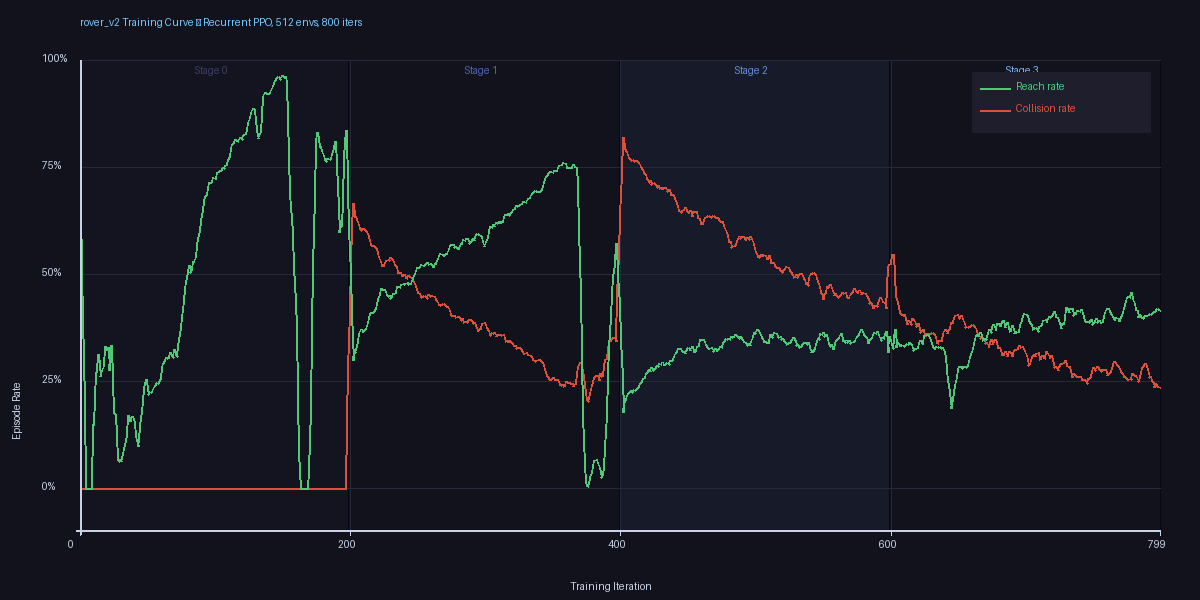
\includegraphics[width=\columnwidth]{rover_v2_training_curve.png}
  \caption{Training curve for \textsc{Rover-v2}. Green: goal-reach rate.
    Red: collision rate. Vertical dashed lines mark curriculum stage boundaries
    (Stage 0$\to$1 at iter~200, 1$\to$2 at iter~400, 2$\to$3 at iter~600).
    Reach drops at each stage transition as obstacle density increases, then
    recovers. Collision rate spikes at Stage~2 when domain randomisation activates,
    then falls to near-zero by Stage~3.}
  \label{fig:training_curve}
\end{figure}

% --------------------------------------------------------------------------- VI. discussion
\section{Discussion}

\subsection{Why 360\textdegree{} Lidar?}

A forward-facing depth camera (the rover's other available sensor) was explicitly
rejected as primary input for several reasons. First, a forward sensor has no
rear coverage: the policy cannot observe obstacles it has passed, leading to
rear-collision failures when reversing and ``commit-to-wrong-side'' errors in narrow
corridors. Second, 72 lidar floats are a compact, homogeneous input well-suited to
recurrent credit assignment; pixel-feature representations require richer
architectures and are harder to normalise across environment variations.
Third, the sim-to-real gap for 2D ray-AABB lidar simulation is narrow: an RPLidar
A2's measurements closely follow the ray-intersection model modulo additive noise
(modelled in training). Rendered depth images carry lighting, texture, and reflection
artefacts absent in training.

\subsection{Why GRU?}

A memoryless MLP baseline was not formally ablated in this work (left for future
work), but qualitative evidence from the drone policy lineage that spawned this
architecture is informative: MLP policies with identical observation spaces exhibited
spinning behaviour in symmetric lidar configurations---equal clearance on both
sides---because they had no history of which direction they had already tried.
The GRU resolves ambiguity via its hidden state, which integrates heading, velocity,
and recent scan history into a soft trajectory memory.

Memory is also important at Stage~3 (slalom gauntlet): the policy must thread a
sequence of offset gaps requiring knowledge of which gap it committed to previously.
A memoryless policy would need to re-solve the local alignment problem at each gap;
the GRU carries the solution forward.

\subsection{The Training--Deployment Gap}

The 45\% training reach / 100\% deployment reach discrepancy (Section~\ref{sec:training})
is practically significant. It implies that stopping training early based on in-training
reach would be premature---the policy at iter~400 (Stage~2, 36\% in-training reach)
may already navigate the named courses reliably, because the named courses are a subset
of the training distribution at a difficulty level the policy has already mastered.

A corollary for practitioners: held-out fixed evaluation courses should be run on
checkpoints throughout training, not just at the final checkpoint. The in-training
metric on the hardest stage will underestimate generalisation on easier held-out
courses.

\subsection{Limitations and Future Work}

\textbf{Sim-to-real.} All results are in simulation. Deploying on a physical rover
requires wiring the ONNX runner to ROS2 \texttt{/cmd\_vel} and validating on the
same six course layouts built in physical space. Based on the narrow sim-to-real gap
for 2D lidar (Section~VI-A) and SITL validation of the companion aerial policy, we
expect acceptable transfer, but do not claim it here.

\textbf{Ablation.} GRU vs.\ MLP, 360\textdegree{} vs.\ forward-only lidar,
curriculum vs.\ no curriculum, and with/without clearance penalty ablations are
planned for a follow-on study. These would firm up the causal claims made qualitatively
above.

\textbf{Dynamic obstacles.} All training obstacles are static. Moving pedestrians or
other robots would require the GRU to track relative velocity, not just position---a
natural extension with a moving-obstacle stage added to the curriculum.

\textbf{Goal sequencing.} The policy takes a single body-frame waypoint. A GPS-based
or graph-search goal sequencer issuing successive waypoints would enable
long-horizon navigation in large environments, cleanly separating global planning
(which can use a map) from reactive avoidance (which does not need one).

% --------------------------------------------------------------------------- VII. conclusion
\section{Conclusion}

We have shown that a recurrent PPO agent with 360\textdegree{} lidar, trained in
30 minutes without demonstrations, achieves 100\% goal-reach with zero collisions
across six qualitatively distinct obstacle courses under realistic sensor noise.
Against a VFH analytic baseline run on identical conditions, the learned policy
achieves a qualitative capability improvement: 120/120 vs.\ 100/120, with VFH
collapsing entirely on dense cluttered fields. The exported 4.6~KB policy runs at
10~Hz on a Jetson Orin Nano, making it immediately deployable on commodity edge
hardware. We release the full training code, course definitions, and evaluation
harness for reproducibility.

% --------------------------------------------------------------------------- references
\begin{thebibliography}{99}

\bibitem{vfh}
J.~Borenstein and Y.~Koren,
``The vector field histogram---fast obstacle avoidance for mobile robots,''
\emph{IEEE Trans.\ Robot.\ Autom.}, vol.~7, no.~3, pp.~278--288, 1991.

\bibitem{vfhplus}
I.~Ulrich and J.~Borenstein,
``VFH+: Reliable obstacle avoidance for fast mobile robots,''
in \emph{Proc.\ IEEE Int.\ Conf.\ Robot.\ Autom.\ (ICRA)}, 1998, pp.~1572--1577.

\bibitem{dwa}
D.~Fox, W.~Burgard, and S.~Thrun,
``The dynamic window approach to collision avoidance,''
\emph{IEEE Robot.\ Autom.\ Mag.}, vol.~4, no.~1, pp.~23--33, 1997.

\bibitem{tai2017virtual}
L.~Tai, G.~Paolo, and M.~Liu,
``Virtual-to-real deep reinforcement learning: Continuous control of mobile robots
for mapless navigation,''
in \emph{Proc.\ IEEE/RSJ Int.\ Conf.\ Intell.\ Robot.\ Syst.\ (IROS)}, 2017,
pp.~31--36.

\bibitem{zhelo2018curiosity}
O.~Zhelo \emph{et al.},
``Curiosity-driven exploration with attentive target driven navigation in robotic
environments,''
\emph{arXiv preprint arXiv:1811.11532}, 2018.

\bibitem{fang2019scene}
Z.~Fang \emph{et al.},
``Scene memory transformer for embodied agents in long-horizon tasks,''
in \emph{Proc.\ IEEE Conf.\ Comput.\ Vis.\ Pattern Recognit.\ (CVPR)}, 2019.

\bibitem{shah2023gnm}
D.~Shah \emph{et al.},
``GNM: A general navigation model to drive any robot,''
in \emph{Proc.\ IEEE Int.\ Conf.\ Robot.\ Autom.\ (ICRA)}, 2023.

\bibitem{mirowski2016learning}
P.~Mirowski \emph{et al.},
``Learning to navigate in complex environments,''
in \emph{Proc.\ Int.\ Conf.\ Learn.\ Represent.\ (ICLR)}, 2017.

\bibitem{zhu2017target}
Y.~Zhu \emph{et al.},
``Target-driven visual navigation in indoor scenes using deep reinforcement learning,''
in \emph{Proc.\ IEEE Int.\ Conf.\ Robot.\ Autom.\ (ICRA)}, 2017, pp.~3357--3364.

\bibitem{kahn2021badgr}
G.~Kahn \emph{et al.},
``BADGR: An autonomous self-supervised learning-based navigation system,''
\emph{IEEE Robot.\ Autom.\ Lett.}, vol.~6, no.~2, pp.~1312--1319, 2021.

\bibitem{bengio2009curriculum}
Y.~Bengio \emph{et al.},
``Curriculum learning,''
in \emph{Proc.\ Int.\ Conf.\ Mach.\ Learn.\ (ICML)}, 2009, pp.~41--48.

\bibitem{tobin2017domain}
J.~Tobin \emph{et al.},
``Domain randomization for transferring deep neural networks from simulation to the
real world,''
in \emph{Proc.\ IEEE/RSJ Int.\ Conf.\ Intell.\ Robot.\ Syst.\ (IROS)}, 2017,
pp.~23--30.

\bibitem{openai2019dexterous}
OpenAI \emph{et al.},
``Solving Rubik's Cube with a Robot Hand,''
\emph{arXiv preprint arXiv:1910.07113}, 2019.

\end{thebibliography}

\end{document}
